% Author: Jan Schaumann <jschauma@netmeister.org>
% $Id: slides.tex,v 1.10 2005/04/04 21:42:02 jschauma Exp $
\special{! TeXDict begin /landplus90{true}store end }

% https://www.dns-oarc.net/oarc/services/porttest

\documentclass[xga]{xdvislides}
\usepackage[landscape]{geometry}
\usepackage{graphics}
\usepackage{graphicx}
\usepackage{colordvi}

\begin{document}
\setfontphv

%%% Headers and footers
\lhead{\slidetitle}                               % default:\lhead{\slidetitle}
\chead{CS615 - Aspects of System Administration}% default:\chead{\relax}
\rhead{Slide \thepage}                       % default:\rhead{\sectiontitle}
\lfoot{\Gray{Popular Services - DNS, SMTP}}% default:\lfoot{\slideauthor}
\cfoot{\relax}                               % default:\cfoot{\relax}
\rfoot{\Gray{\today}}

\vspace*{\fill}
\begin{center}
	\Hugesize
		CS615 - Aspects of System Administration\\ [1em]
		Popular Services - DNS, SMTP\\ [1em]
	\hspace*{5mm}\blueline\\ [1em]
	\Normalsize
		Department of Computer Science\\
		Stevens Institute of Technology\\
		Jan Schaumann\\
		\verb+jschauma@stevens.edu+ \\
		\verb+http://www.cs.stevens.edu/~jschauma/615/+
\end{center}
\vspace*{\fill}

\subsection{In the beginning...}
\vspace*{\fill}
\begin{center}
	\includegraphics[scale=0.8]{pics/2computers.eps} \\
\end{center}
\vspace*{\fill}

\subsection{In the beginning...}
\vspace*{\fill}
\begin{center}
	\includegraphics[scale=0.8]{pics/2computers-nic.eps} \\
\end{center}
\vspace*{\fill}

\subsection{In the beginning...}
\vspace*{\fill}
\begin{center}
	\includegraphics[scale=0.8]{pics/3computers.eps} \\
\end{center}
\vspace*{\fill}

\subsection{In the beginning...}
\vspace*{\fill}
\begin{center}
	\includegraphics[scale=0.8]{pics/3computers-1.eps} \\
\end{center}
\vspace*{\fill}

\subsection{In the beginning...}
\vspace*{\fill}
\begin{center}
	\includegraphics[scale=0.8]{pics/3computers-2.eps} \\
\end{center}
\vspace*{\fill}

\subsection{In the beginning...}
\begin{verbatim}
# Host Database
# This file should contain the addresses and aliases
# for local hosts that share this file.
#
127.0.0.1               localhost localhost.
#
# RFC 1918 specifies that these networks are "internal".
# 10.0.0.0      10.255.255.255
# 172.16.0.0    172.31.255.255
# 192.168.0.0   192.168.255.255
10.0.0.1	UCLA-TEST
10.0.0.2	SRI-SPRM
10.0.0.4	UTAH-CS
\end{verbatim}


\subsection{But then...}
\vspace*{\fill}
\begin{center}
	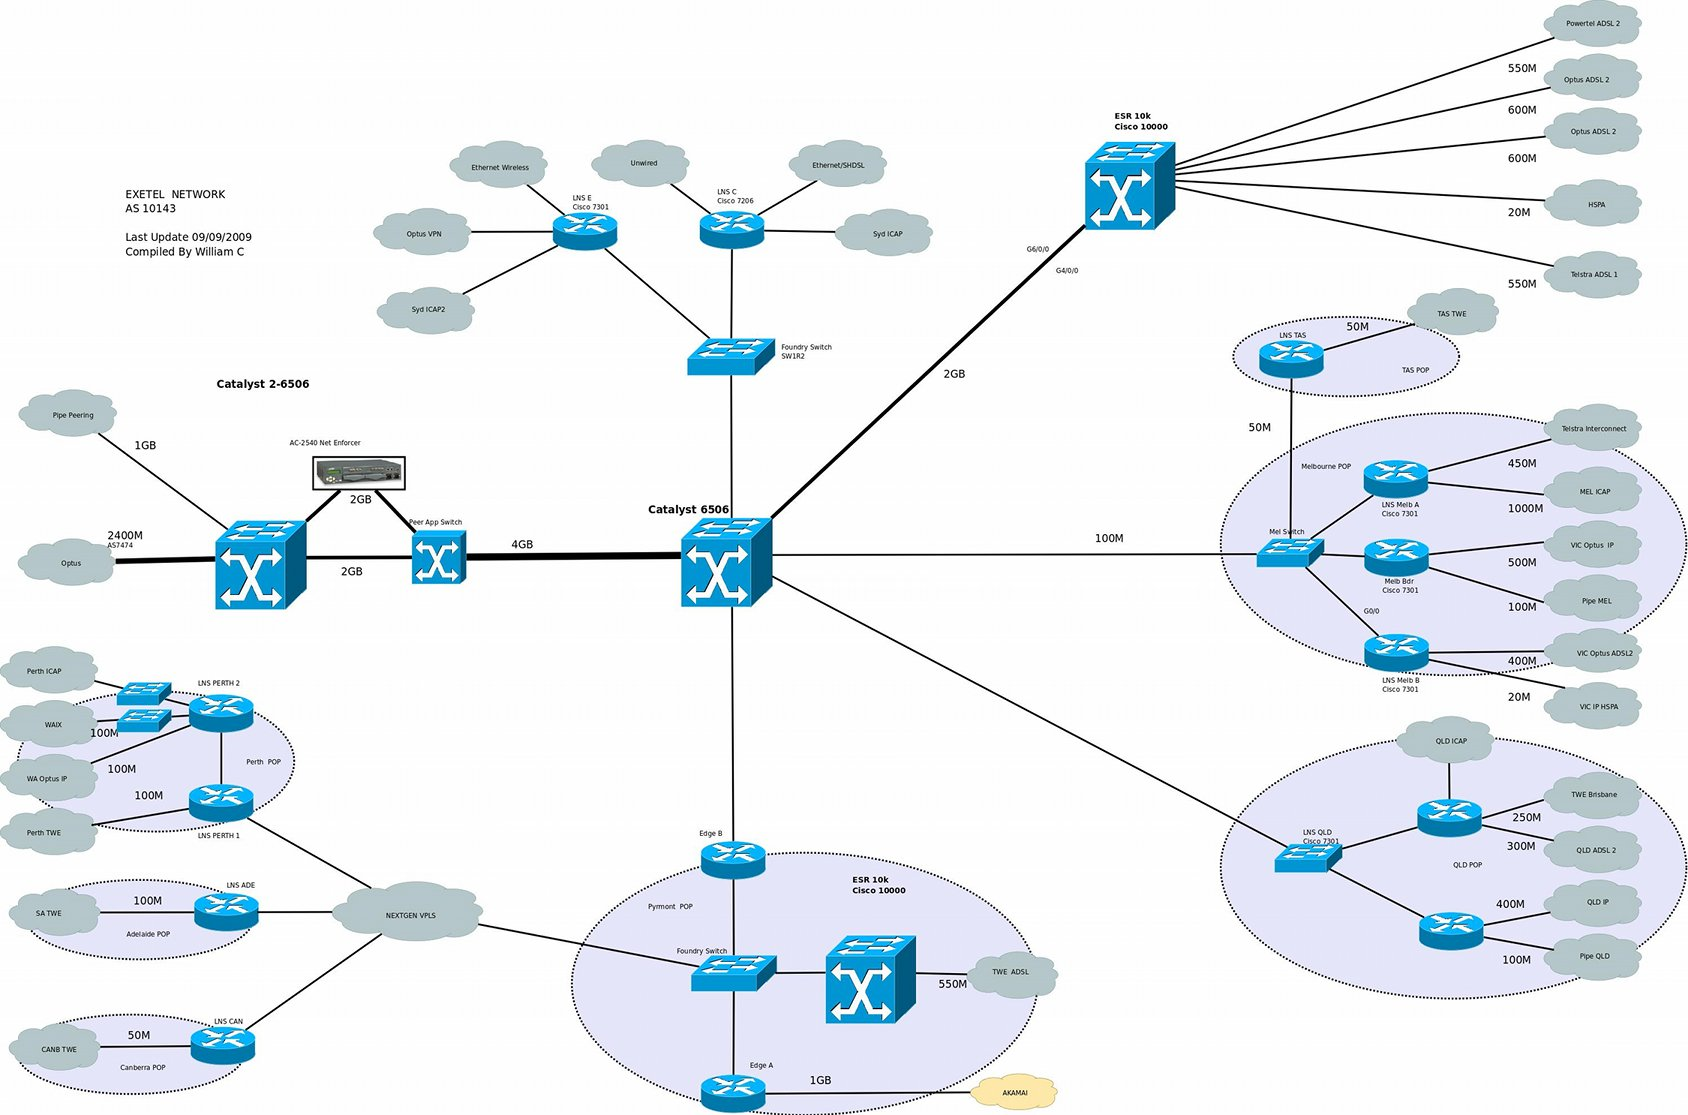
\includegraphics[scale=0.3]{pics/routed.eps} \\
\end{center}
\vspace*{\fill}

\subsection{The Domain Name System}
\vspace{.5in}
\begin{center}
	\Huge
	Computers like numbers. \\
\vspace{.5in}
\begin{verbatim}
         10011011111101100101100110011111
\end{verbatim}
\end{center}
\Normalsize

\subsection{The Domain Name System}
\vspace{.5in}
\begin{center}
	\Huge
	Computers like numbers. \\
\vspace{.5in}
\begin{verbatim}
      10011011  11110110  01011001  10011111

        155   .   246   .    89   .   159
\end{verbatim}
\end{center}
\Normalsize

\subsection{The Domain Name System}
\vspace{.5in}
\begin{center}
	\Huge
	People like names. \\
\vspace{.5in}
\verb+ash.cs.stevens-tech.edu+
\end{center}
\Normalsize


\subsection{The Domain Name System}
\vspace*{\fill}
\begin{center}
	
\includegraphics[scale=0.6]{pics/phonebook.eps}
\end{center}
\vspace*{\fill}

\subsection{The New Phonebook is here!}
\vspace*{\fill}
\begin{center}
	\verb+http://is.gd/XXp2sC+ \\
	\addvspace{.5in}
	\verb+wget -q -O - http://is.gd/XXp2sC | grep -c "^HOST"+
\end{center}
\vspace*{\fill}

\subsection{DNS: A distributed database}
\vspace*{\fill}
\begin{center}
	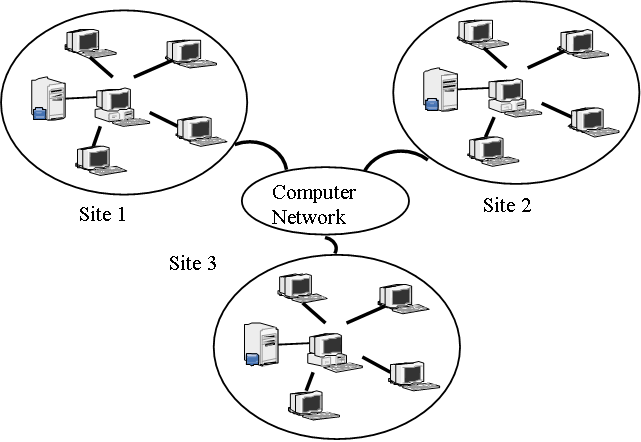
\includegraphics[scale=0.75]{pics/distributed-database.eps}
\end{center}
\vspace*{\fill}

\subsection{The Domain Name Space}
\vspace{.5in}
\begin{center}
	\Huge
	The domain name space consists of a tree of {\em domain} names.
\end{center}
\Normalsize

\subsection{DNS: A hierarchical system}
\vspace*{\fill}
\begin{center}
	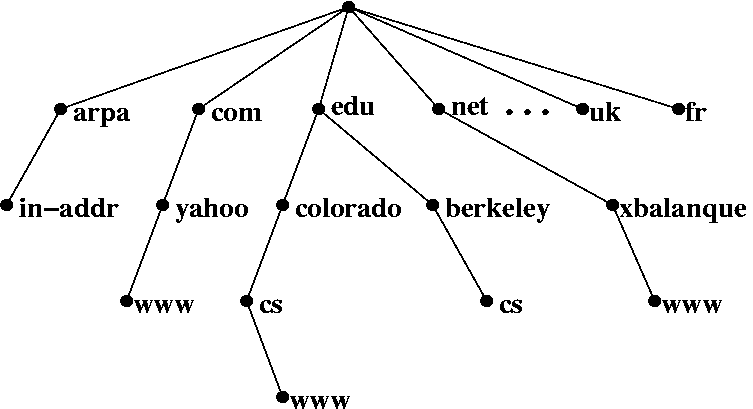
\includegraphics[scale=0.75]{pics/hierarchical-dns.eps}
\end{center}
\vspace*{\fill}

\subsection{The Domain Name Space}
\vspace{.5in}
\begin{center}
	\Huge
	The domain name space consists of a tree of {\em domain} names. \\
	\vspace{.5in}
	A subtree divides into {\em zones}.
\end{center}
\Normalsize

\subsection{The Domain Name Space}
\vspace{.5in}
\begin{center}
	\Huge
	The domain name space consists of a tree of {\em domain} names. \\
	\vspace{.5in}
	A subtree divides into {\em zones}. \\
	\vspace{.5in}
	Each node may contain {\em resource records}.
\end{center}
\Normalsize

\subsection{The Domain Name Space}
\vspace*{\fill}
\begin{center}
	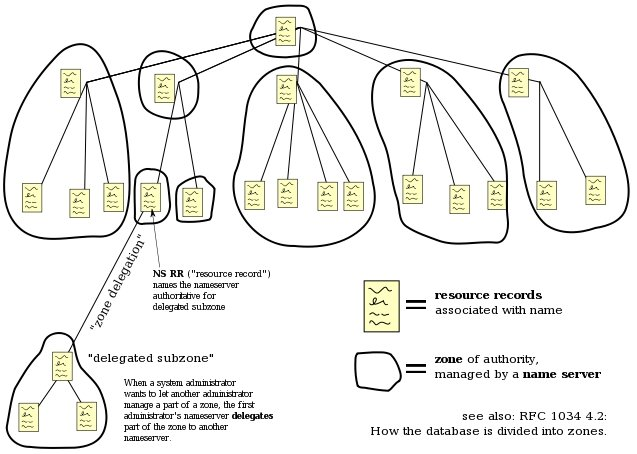
\includegraphics[scale=0.74]{pics/dns-space.eps}
\end{center}
\vspace*{\fill}

\subsection{Domain Names}
\vspace{.5in}
\begin{center}
	\Huge
	\verb+ash.cs.stevens-tech.edu+ \\
	\vspace{.5in}
	Domain Names are read from right to left and components separated by a ``\verb+.+''.
\end{center}
\Normalsize

\subsection{Domain Names}
\vspace{.5in}
\begin{center}
	\Huge
	\verb+ash.cs.stevens-tech.edu.+ \\
	\vspace{.5in}
	The {\em root} is known as ``\verb+.+'', but is usually left out.
\end{center}
\Normalsize

\subsection{Domain Names}
\vspace{.5in}
\begin{center}
	\Huge
	\verb+ash.cs.stevens-tech.+{\bf edu}\verb+.+ \\
	\vspace{.5in}
	There is a small number of {\em top level domains}.
\end{center}
\Normalsize

\subsection{Domain Names}
\vspace{.5in}
\begin{center}
	\Huge
	\verb+ash.cs.stevens-tech.+{\bf edu}\verb+.+ \\
	\vspace{.5in}
	There is a number of {\em top level domains}. \\
	\vspace{.5in}
	\verb+ftp://rs.internic.net/domain/root.zone+ \\
	\vspace{.25in}
	\Normalsize
	\verb+https://en.wikipedia.org/wiki/List_of_Internet_top-level_domains+
\end{center}
\Normalsize


\subsection{Domain Names}
\vspace{.5in}
\begin{center}
	\Huge
	\verb+ash.cs.+{\bf stevens-tech}\verb+.edu.+ \\
	\vspace{.5in}
	Each {\em domain} can be divided into any number of {\em sub domains}.
\end{center}
\Normalsize

\subsection{Domain Names}
\vspace{.5in}
\begin{center}
	\Huge
	\verb+ash.+{\bf cs}\verb+.stevens-tech.edu.+ \\
	\vspace{.5in}
	Each {\em domain} can be divided into any number of {\em sub domains}.
\end{center}
\Normalsize

\subsection{Domain Names}
\vspace{.5in}
\begin{center}
	\Huge
	{\bf ash}\verb+.cs.stevens-tech.edu.+ \\
	\vspace{.5in}
	The left-most component of a domain name may be a {\em hostname}.
\end{center}
\Normalsize

\subsection{Fully Qualified Domain Names}
\vspace{.5in}
\begin{center}
	\Huge
	\verb+ash.cs.stevens-tech.edu.+ \\
	\vspace{.5in}
	A {\em hostname} with a domain name is known as a {\em FQDN}.
\end{center}
\Normalsize


\subsection{DNS servers come in two flavors}
\vspace*{\fill}
\begin{center}
	\begin{tabular}{ c c c }
	
\includegraphics[scale=1.5]{pics/vanilla.eps} & \hspace{.5in} & 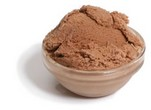
\includegraphics[scale=1.5]{pics/chocolate.eps} \\
	\hspace{.3in} \Huge Authoritative & & \hspace{.3in} \Huge Recursive \\
	\hspace{.3in} \Huge Nameservers & & \hspace{.3in} \Huge Nameservers \\
	\end{tabular}
\end{center}
\vspace*{\fill}

\subsection{Hostname resolution}
Resolution on a recursive nameserver (aka {\em resolver}) involves a number of queries:
\vspace{.5in}
\begin{verbatim}
$ nslookup ash.cs.stevens-tech.edu
Server:         127.0.0.1
Address:        127.0.0.1#53

Non-authoritative answer:
Name:   ash.cs.stevens-tech.edu
Address: 155.246.89.159

$
\end{verbatim}

\subsection{Hostname resolution}
Resolution on a {\em resolver} involves a number of queries:
\begin{verbatim}
18:39:27.186778 IP panix.netmeister.org.62105 > i.root-servers.net.domain:
        11585 [1au] A? ash.cs.stevens-tech.edu. (52)
18:39:27.446190 IP i.root-servers.net.domain > panix.netmeister.org.62105:
        11585- 0/8/8 (494)
18:39:27.446994 IP panix.netmeister.org.53168 > a.gtld-servers.net.domain:
        46575 [1au] A? ash.cs.stevens-tech.edu. (52)
18:39:27.481565 IP a.gtld-servers.net.domain > panix.netmeister.org.53168:
        46575- 0/6/3 (609)
18:39:27.481998 IP panix.netmeister.org.41071 > nrac.stevens-tech.edu.domain:
        24322 [1au] A? ash.cs.stevens-tech.edu. (52)
18:39:27.486035 IP nrac.stevens-tech.edu.domain > panix.netmeister.org.41071:
        24322*- 1/2/3 A[|domain]
\end{verbatim}
\Normalsize

\subsection{Hostname resolution}
Resolution on a {\em resolver} involves a number of queries:
\begin{verbatim}
$ host -t ns .
. name server I.ROOT-SERVERS.NET.
. name server D.ROOT-SERVERS.NET.
. name server C.ROOT-SERVERS.NET.
. name server M.ROOT-SERVERS.NET.
. name server F.ROOT-SERVERS.NET.
. name server A.ROOT-SERVERS.NET.
. name server E.ROOT-SERVERS.NET.
. name server L.ROOT-SERVERS.NET.
. name server H.ROOT-SERVERS.NET.
. name server J.ROOT-SERVERS.NET.
. name server B.ROOT-SERVERS.NET.
. name server G.ROOT-SERVERS.NET.
. name server K.ROOT-SERVERS.NET.
$
\end{verbatim}

\subsection{Hostname resolution}
Resolution on a {\em resolver} involves a number of queries:
\begin{verbatim}
$ dig -t ns edu.
[...]
;; ANSWER SECTION:
edu.                    172800  IN      NS      l.edu-servers.net.
edu.                    172800  IN      NS      f.edu-servers.net.
edu.                    172800  IN      NS      c.edu-servers.net.
edu.                    172800  IN      NS      g.edu-servers.net.
edu.                    172800  IN      NS      a.edu-servers.net.
edu.                    172800  IN      NS      d.edu-servers.net.

;; ADDITIONAL SECTION:
c.edu-servers.net.      36626   IN      A       192.26.92.30
d.edu-servers.net.      13274   IN      A       192.31.80.30
l.edu-servers.net.      36626   IN      A       192.41.162.30
[...]
$
\end{verbatim}
\Normalsize

\subsection{Hostname resolution}
Resolution on a {\em resolver} involves a number of queries:
\begin{verbatim}
$ dig @c.edu-servers.net -t ns stevens.edu.
[...]
;; AUTHORITY SECTION:
stevens.edu.            172800  IN      NS      nrac.stevens-tech.edu.
stevens.edu.            172800  IN      NS      sitult.stevens-tech.edu.

;; ADDITIONAL SECTION:
nrac.stevens-tech.edu.  172800  IN      A       155.246.1.21
sitult.stevens-tech.edu. 172800 IN      A       155.246.1.20
[...]
$
\end{verbatim}

\subsection{Hostname resolution}
\vspace*{\fill}
\begin{center}
	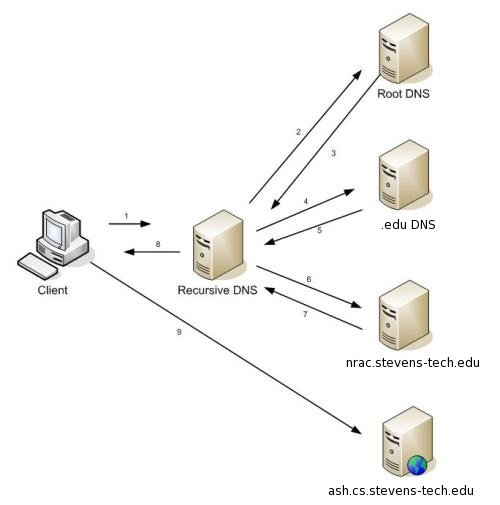
\includegraphics[scale=0.9]{pics/resolution.eps}
\end{center}
\vspace*{\fill}


\subsection{Hostname resolution}
Resolution on a {\em resolver} involves a number of queries:
\begin{verbatim}
$ nslookup ash.cs.stevens-tech.edu
Server:         127.0.0.1
Address:        127.0.0.1#53

Non-authoritative answer:
Name:   ash.cs.stevens-tech.edu
Address: 155.246.89.159

$
\end{verbatim}

\subsection{Hostname resolution}
\vspace*{\fill}
\begin{center}
	
\includegraphics[scale=0.4]{pics/chicken-egg.eps} \\
	\vspace*{\fill}
\end{center}

\subsection{Hostname resolution}
\vspace*{\fill}
\begin{center}
	
\includegraphics[scale=0.4]{pics/chicken-egg.eps} \\
	\addvspace{.2in}
	\verb+$ ftp -o - ftp.internic.net:/domain/db.cache | more+
	\vspace*{\fill}
\end{center}

\subsection{Operation Global Blackout}
\vspace*{\fill}
\begin{center}
	
\includegraphics[scale=0.8]{pics/anonymous.eps} \\
	\addvspace{.2in}
	\verb+http://pastebin.com/XZ3EGsbc+ \\
	\addvspace{.1in}
	\small
	Btw, read this, too: \verb+https://en.wikipedia.org/wiki/Guy_Fawkes+
\end{center}
\vspace*{\fill}

\subsection{DNS: A distributed system}
\vspace{.5in}
\begin{center}
	\Huge
	There are 13 \verb+root+ servers. \\
\end{center}
\Normalsize

\subsection{DNS: A distributed system}
\vspace{.5in}
\begin{center}
	\Huge
	There are 13 \verb+root+ servers. \\
	\vspace{.5in}
	Except... there are more.
\end{center}
\Normalsize

\subsection{DNS: A distributed system}
\vspace{.5in}
\begin{center}
	\Huge
	There are 13 \verb+root+ {\em authorities}. \\
\end{center}
\Normalsize

\subsection{DNS: A distributed system}
\vspace{.5in}
\begin{center}
	\Huge
	There are 13 \verb+root server+ {\em addresses}. \\
\end{center}
\Normalsize

\subsection{DNS: A distributed system}
\vspace{.5in}
\begin{center}
	\Huge
	There are hundreds of \verb+root+ servers. \\
\end{center}
\Normalsize

\subsection{DNS: A distributed system}
\vspace*{\fill}
\begin{center}
	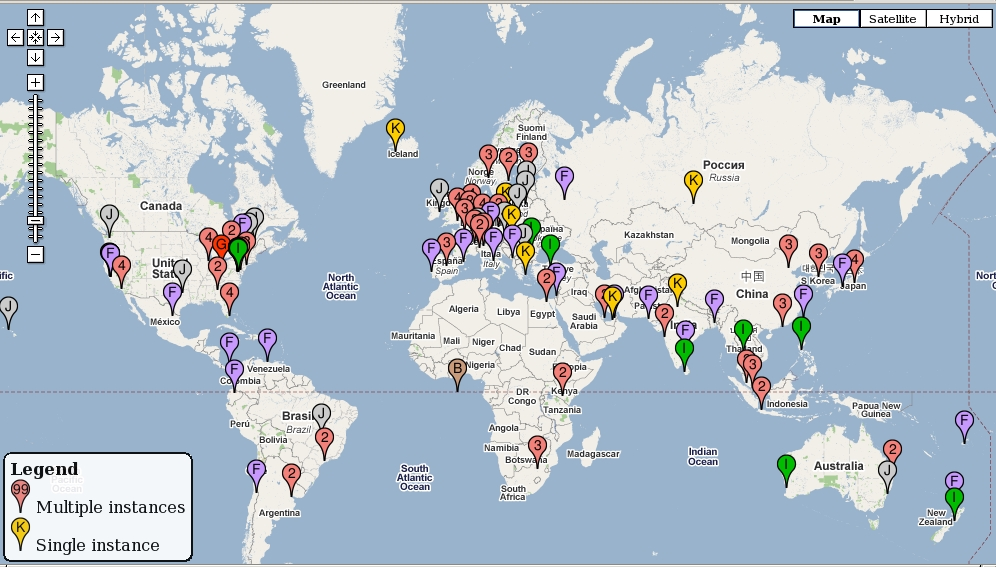
\includegraphics[scale=0.5]{pics/root-servers.eps}
\end{center}
\vspace*{\fill}

\subsection{Operation Global Blackout}
\vspace*{\fill}
\begin{center}
	
\includegraphics[scale=0.8]{pics/anonymous-tweet.eps} \\
\end{center}
\vspace*{\fill}

\subsection{DNS: A distributed database}
\vspace*{\fill}
\begin{center}
	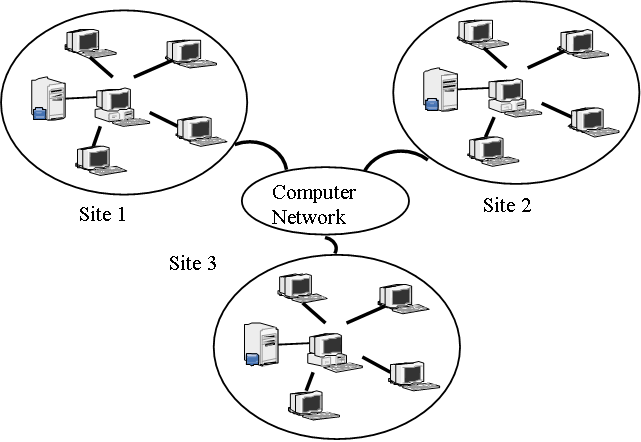
\includegraphics[scale=0.75]{pics/distributed-database.eps}
\end{center}
\vspace*{\fill}


\subsection{DNS Resource Records}
\begin{itemize}
	\item {\em NS} -- an authoritative name server
	\item {\em CNAME} -- the canonical name for an alias
	\item {\em SOA} -- marks the start of a zone of authority
	\item {\em PTR} -- a domain name pointer
	\item {\em HINFO} -- host information
	\item {\em MX} -- mail exchange
	\item {\em TXT} text strings
	\item ...
\end{itemize}

\subsection{DNS Resource Records}
\begin{verbatim}
$ host ash.cs.stevens-tech.edu
ash.cs.stevens-tech.edu has address 155.246.89.159
ash.cs.stevens-tech.edu mail is handled by 0 guinness.cs.stevens-tech.edu.
$
\end{verbatim}

\subsection{DNS Resource Records}
\begin{verbatim}
$ host a.gtld-servers.net
a.gtld-servers.net has address 192.5.6.30
a.gtld-servers.net has IPv6 address 2001:503:a83e::2:30
$ host -t ptr 2001:503:a83e::2:30
0.3.0.0.2.0.0.0.0.0.0.0.0.0.0.0.0.0.0.0.e.3.8.a.3.0.5.0.1.0.0.2.ip6.arpa
    domain name pointer a.gtld-servers.net.
$ host -t ptr 192.5.6.30
30.6.5.192.in-addr.arpa domain name pointer a.gtld-servers.net.
\end{verbatim}

\subsection{Creative uses of DNS Resource Records}
\begin{itemize}
	\item identifying sources of SPAM (see next section)
	\item find ASN numbers by IP addresses: \\
		\verb|dig +short 159.89.246.155.origin.asn.cymru.com TXT|
	\item check a resolvers source port randomization (to help
		mitigate DNS Cache Poisoning attacks): \\
		\verb|dig +short porttest.dns-oarc.net TXT|
	\item using DNS to publish SSH key fingerprints (RFC4255,
ssh\_config(5) \verb+VerifyHostKeyDNS+; for best results combine with DNSSEC): \\
		\verb|dig +short ftp.netbsd.org SSHFP| \\
		\begin{verbatim}
ssh -o "VerifyHostKeyDNS yes" ftp.netbsd.org
The authenticity of host 'ftp.netbsd.org (199.233.217.249)' can't be established.
RSA key fingerprint is b9:04:78:bc:aa:1a:09:34:f9:17:e6:2e:ef:9c:3f:ab.
Matching host key fingerprint found in DNS.
Are you sure you want to continue connecting (yes/no)?
\end{verbatim}
\end{itemize}

\newpage
\vspace*{\fill}
\begin{center}
    \Hugesize
        Hooray! \\ [1em]
    \hspace*{5mm}
    \blueline\\
    \hspace*{5mm}\\
        5 Minute Break
\end{center}
\vspace*{\fill}


\newpage
\vspace*{\fill}
\begin{center}
	\Hugesize
		Popular Services \\ [1em]
	\hspace*{5mm}
	\blueline\\
	\hspace*{5mm}\\
		Simple Mail Transfer Protocol
\end{center}
\vspace*{\fill}

\subsection{Email... still popular}
\begin{itemize}
	\item {\bf 90 trillion} – The number of emails sent on the Internet in 2009.
	\item {\bf 247 billion} – Average number of email messages per day.
	\item {\bf 1.4 billion} – The number of email users worldwide.
	\item {\bf 100 million} – New email users since the year before.
	\item {\bf 81\%} – The percentage of emails that were spam.
	\item {\bf 92\%} – Peak spam levels late in the year.
	\item {\bf 24\%} – Increase in spam since last year.
	\item {\bf 200 billion} – The number of spam emails per day (assuming 81\% are spam).
\end{itemize}

\subsection{Sending email}
\begin{verbatim}
$ mail -s "Act I, Scene I" jschauma@cs.stevens.edu
When shall we three meet again?
In thunder lightning or in rain?
.
EOT
$
\end{verbatim}

\subsection{Receiving mail}
\begin{verbatim}
Date: Sun, 27 Mar 2011 18:54:04 -0400 (EDT)
From: Jan Schaumann <jschauma@netmeister.org>
To: jschauma@cs.stevens.edu
Subject: Act I, Scene I

When shall we three meet again
In thunder lightning or in rain?

\end{verbatim}

\subsection{In more detail...}
Finding the right mail server to talk to:
\begin{verbatim}
166.84.7.99.57149 > 166.84.67.2.53: 61301+ MX? cs.stevens.edu. (32)
166.84.67.2.53 > 166.84.7.99.57149: 61301 4/2/4 MX[|domain]
166.84.7.99.57148 > 166.84.67.2.53: 61302+ A? stevens.edu.s9a1.psmtp.com. (44)
166.84.67.2.53 > 166.84.7.99.57148: 61302 1/8/8 (343)
166.84.7.99.57147 > 166.84.67.2.53: 61303+ AAAA? stevens.edu.s9a1.psmtp.com. (44)
166.84.67.2.53 > 166.84.7.99.57147: 61303 0/1/0 (121)
166.84.7.99.57146 > 166.84.67.2.53: 61304+ A? stevens.edu.s9a2.psmtp.com. (44)
166.84.67.2.53 > 166.84.7.99.57146: 61304 1/8/8 (343)
166.84.7.99.57145 > 166.84.67.2.53: 61305+ AAAA? stevens.edu.s9a2.psmtp.com. (44)
166.84.67.2.53 > 166.84.7.99.57145: 61305 0/1/0 (121)
166.84.7.99.57144 > 166.84.67.2.53: 61306+ A? stevens.edu.s9b1.psmtp.com. (44)
166.84.67.2.53 > 166.84.7.99.57144: 61306 1/8/8 (343)
166.84.7.99.57143 > 166.84.67.2.53: 61307+ AAAA? stevens.edu.s9b1.psmtp.com. (44)
166.84.67.2.53 > 166.84.7.99.57143: 61307 0/1/0 (121)
\end{verbatim}
\Normalsize

\subsection{In more detail...}
Making the connection:
\begin{verbatim}
166.84.7.99.56525 > 74.125.148.10.25: S 74074538:74074538(0)
74.125.148.10.25 > 166.84.7.99.56525: S 3395438539:3395438539(0) ack 74074539
166.84.7.99.56525 > 74.125.148.10.25: . ack 1
74.125.148.10.25 > 166.84.7.99.56525: P 1:167(166) ack 1
166.84.7.99.56525 > 74.125.148.10.25: P 1:28(27) ack 167
74.125.148.10.25 > 166.84.7.99.56525: . ack 28
74.125.148.10.25 > 166.84.7.99.56525: P 167:234(67) ack 28
166.84.7.99.56525 > 74.125.148.10.25: P 28:65(37) ack 234
74.125.148.10.25 > 166.84.7.99.56525: P 234:242(8) ack 65
166.84.7.99.56525 > 74.125.148.10.25: P 65:100(35) ack 242
[...]
166.84.7.99.56525 > 74.125.148.10.25: P 506:512(6) ack 275
166.84.7.99.56525 > 74.125.148.10.25: F 512:512(0) ack 275
74.125.148.10.25 > 166.84.7.99.56525: . ack 512
74.125.148.10.25 > 166.84.7.99.56525: P 275:296(21) ack 513
74.125.148.10.25 > 166.84.7.99.56525: F 296:296(0) ack 513
\end{verbatim}
\Normalsize

\subsection{In more detail...}
Receiving the mail:
\begin{verbatim}
74.125.149.240.57878 > 166.84.7.99.25: S 1146367109:1146367109(0)
166.84.7.99.25 > 74.125.149.240.57878: S 244504993:244504993(0) ack 1146367110
74.125.149.240.57878 > 166.84.7.99.25: . ack 1
166.84.7.99.57130 > 166.84.67.2.53: 51274+ PTR? 240.149.125.74.in-addr.arpa. (45)
166.84.67.2.53 > 166.84.7.99.57130: 51274 1/6/6 (300)
166.84.7.99.57129 > 166.84.67.2.53: 51275+ AAAA? na3sys009aog116.obsmtp.com. (44)
166.84.67.2.53 > 166.84.7.99.57129: 51275 0/1/0 (121)
166.84.7.99.57128 > 166.84.67.2.53: 51276+ A? na3sys009aog116.obsmtp.com. (44)
166.84.67.2.53 > 166.84.7.99.57128: 51276 1/8/8 (343)
166.84.7.99.25 > 74.125.149.240.57878: P 1:41(40) ack 1
74.125.149.240.57878 > 166.84.7.99.25: . ack 41
74.125.149.240.57878 > 166.84.7.99.25: P 1:34(33) ack 41
166.84.7.99.25 > 74.125.149.240.57878: P 41:67(26) ack 34
74.125.149.240.57878 > 166.84.7.99.25: P 34:71(37) ack 67
166.84.7.99.25 > 74.125.149.240.57878: P 67:81(14) ack 71
[...]
\end{verbatim}

\subsection{In more detail...}
Receiving the mail:
\begin{verbatim}
166.84.7.99.57127 > 166.84.67.2.53: 51277+ A? na3sys009aog116.obsmtp.com. (44)
166.84.67.2.53 > 166.84.7.99.57127: 51277 1/8/8 (343)
166.84.7.99.57126 > 166.84.67.2.53: 51278+ A? 240.149.125.74.sbl.spamhaus.org. (49)
166.84.67.2.53 > 166.84.7.99.57126: 51278 NXDomain 0/1/0 (105)
166.84.7.99.57125 > 166.84.67.2.53: 51279+ A? 240.149.125.74.list.dsbl.org. (46)
166.84.7.99.25 > 74.125.149.240.57878: . ack 106
166.84.7.99.57124 > 198.7.0.5.53: 51279+ A? 240.149.125.74.list.dsbl.org. (46)
166.84.7.99.57125 > 166.84.67.2.53: 51279+ A? 240.149.125.74.list.dsbl.org. (46)
166.84.7.99.57124 > 198.7.0.5.53: 51279+ A? 240.149.125.74.list.dsbl.org. (46)
166.84.7.99.57123 > 166.84.67.2.53: 51280+ A? 240.149.125.74.bl.spamcop.net. (47)
166.84.67.2.53 > 166.84.7.99.57123: 51280 NXDomain 0/1/0 (100)
166.84.7.99.25 > 74.125.149.240.57878: P 81:95(14) ack 106
74.125.149.240.57878 > 166.84.7.99.25: . ack 95
74.125.149.240.57878 > 166.84.7.99.25: P 106:112(6) ack 95
[...]
\end{verbatim}

\subsection{In more detail...}
Receiving the mail:
\begin{verbatim}
[...]
166.84.7.99.25 > 74.125.149.240.57878: P 95:132(37) ack 112
74.125.149.240.57878 > 166.84.7.99.25: . ack 132
74.125.149.240.57878 > 166.84.7.99.25: P 112:1216(1104) ack 132
166.84.7.99.25 > 74.125.149.240.57878: . ack 1216
74.125.149.240.57878 > 166.84.7.99.25: P 1216:1286(70) ack 132
166.84.7.99.25 > 74.125.149.240.57878: P 132:169(37) ack 1286
74.125.149.240.57878 > 166.84.7.99.25: P 1286:1292(6) ack 169
166.84.7.99.25 > 74.125.149.240.57878: P 169:184(15) ack 1292
166.84.7.99.25 > 74.125.149.240.57878: F 184:184(0) ack 1292
74.125.149.240.57878 > 166.84.7.99.25: F 1292:1292(0) ack 184
74.125.149.240.57878 > 166.84.7.99.25: . ack 185
166.84.7.99.25 > 74.125.149.240.57878: . ack 1293
\end{verbatim}
\Normalsize

\subsection{In less detail...}
\newcommand{\smallish}{\fontsize{16}{16}\selectfont}
\begin{verbatim}
$ host -t mx cs.stevens.edu
cs.stevens.edu mail is handled by 20 stevens.edu.s9a2.psmtp.com.
cs.stevens.edu mail is handled by 30 stevens.edu.s9b1.psmtp.com.
cs.stevens.edu mail is handled by 10 stevens.edu.s9a1.psmtp.com.
cs.stevens.edu mail is handled by 40 stevens.edu.s9b2.psmtp.com.
$
\end{verbatim}
\Normalsize

\subsection{In less detail...}
\begin{verbatim}
$ dig stevens.edu.s9a1.psmtp.com.
;; ANSWER SECTION:
stevens.edu.s9a1.psmtp.com. 13748 IN    A       74.125.148.10

;; AUTHORITY SECTION:
psmtp.com.              6078    IN      NS      ns2.ns.postini.com.
psmtp.com.              6078    IN      NS      ns1.ns.postini.com.
psmtp.com.              6078    IN      NS      ns4.ns.postini.com.
psmtp.com.              6078    IN      NS      ns3.ns.postini.com.

;; ADDITIONAL SECTION:
ns1.google.com.         321436  IN      A       216.239.32.10
ns2.google.com.         279978  IN      A       216.239.34.10
ns3.google.com.         301560  IN      A       216.239.36.10
ns4.google.com.         286535  IN      A       216.239.38.10
[...]
$
\end{verbatim}

\subsection{In less detail...}
\smallish
\begin{verbatim}
$ telnet stevens.edu.s9a1.psmtp.com 25
Trying 74.125.148.10...
Connected to stevens.edu.s9a1.psmtp.com.
Escape character is '^]'.
220 Postini ESMTP 202 y6_37_0c5 ready.  CA Business and Professions Code
Section 17538.45 forbids use of this system for unsolicited electronic
mail advertisements.
helo panix.netmeister.org
250 Postini says hello back
mail from: <jschauma@netmeister.org>
250 Ok
rcpt to: <jschauma@cs.stevens.edu>
250 Ok
data
354 Feed me
Subject: Act I, Scene I

When shall we three meet again
In thunder, lightning or in rain?
.
250 Thanks
quit
221 Catch you later
Connection closed by foreign host.
\end{verbatim}
\Normalsize

\subsection{SMTP Codes}
SMTP codes consist of three digits in five classes:
\begin{itemize}
	\item {\bf 1xx} --  Mail server has accepted the command, but does not yet
		take any action. A confirmation message is required.
	\item {\bf 2xx} --  Mail server has completed the task successfully
		without errors.
	\item {\bf 3xx} --  Mail server has understood the request, but requires
		further information to complete it.
	\item {\bf 4xx} --  Mail server has encountered a temporary failure. If
		the command is repeated without any change, it might be
		completed. Try again, it may help!
	\item {\bf 5xx} --  Mail server has encountered a fatal error. Your
		request can't be processed.
\end{itemize}

\subsection{Anatomy of an email message}
\begin{verbatim}
Date: Sun, 18 Mar 2012 22:47:36 -0400 (EDT)
From: jschauma@cs.stevens.edu
To: undisclosed-recipients: ;
Subject: Act I, Scene I

When shall we three meet again
In thunder lightning or in rain?

\end{verbatim}

\subsection{Anatomy of an email message}
\small
\begin{verbatim}
From jschauma@cs.stevens.edu  Sun Mar 18 22:48:09 2012
Return-Path: jschauma@cs.stevens.edu
X-Original-To: jschauma@netmeister.org
Delivered-To: jschauma@netmeister.org
Received: by panix.netmeister.org (Postfix, from userid 1004)
        id 93A29356BC1; Sun, 18 Mar 2012 22:48:09 -0400 (EDT)
Received: from na3sys009aog108.obsmtp.com (na3sys009aog108.obsmtp.com [74.125.149.199])
        by panix.netmeister.org (Postfix) with SMTP id 69B91356BBB
        for <jschauma@netmeister.org>; Sun, 18 Mar 2012 22:47:49 -0400 (EDT)
Received: from warp.stevens.edu ([155.246.14.14]) by na3sys009aob108.postini.com ([74.125.148.12])
        with SMTP ID DSNKT2aeVJEJy0AYQcjXfWII8P62lyoYXAFm@postini.com; Sun, 18 Mar 2012 19:48:08 PDT
Received: from psmtp.com (na3sys009amx209.postini.com [74.125.149.49])
        by warp.stevens.edu (Postfix) with SMTP id 168646041A
        for <jschauma@cs.stevens.edu>; Sun, 18 Mar 2012 22:47:36 -0400 (EDT)
Received: from eva.srcit.stevens-tech.edu ([155.246.89.108]) by na3sys009amx209.postini.com
        ([74.125.148.10]) with SMTP; Sun, 18 Mar 2012 21:47:39 CDT
Subject: Act I, Scene I
X-pstn-neptune: 0/0/0.00/0
X-pstn-levels:     (S:30.88262/99.90000 CV:99.9000 FC:95.5390 LC:95.5390
R:95.9108 P:95.9108
        M:97.0282 C:98.6951 )
X-pstn-dkim: 0 skipped:no-from
Message-ID: <2615178024788798087302160308530@psmtp.com>
X-pstn-settings: 3 (1.0000:1.0000) s cv gt3 gt2 gt1
X-pstn-addresses: from <jschauma@cs.stevens.edu> [db-null]
Date: Sun, 18 Mar 2012 22:47:36 -0400 (EDT)
From: jschauma@cs.stevens.edu
To: undisclosed-recipients: ;

When shall we three meet again
In thunder, lightning or in rain?
\end{verbatim}
\Normalsize

\subsection{Anatomy of an email message}
An email consists of:
\begin{itemize}
	\item mandatory headers (such as "From ", "Delivered-To: ", ...)
	\item optional headers (such as "From: ", "To: ", "Subject: ", ...)
	\item the (optional) body of the message
\end{itemize}

\subsection{The Mail System}
Divided into
\begin{itemize}
	\item {\em Mail User Agent} or MUA, such as {\em mutt}
	\item {\em Mail Transfer Agent} or MTA, such as {\em postfix}
	\item {\em Mail Delivery Agent} or MDA, such as {\em procmail}
	\item {\em Access Agent} providing access via {\em POP}, {\em IMAP} etc.
\end{itemize}

\subsection{HW4}
\verb+http://www.cs.stevens.edu/~jschauma/615/s12-hw4.html+

\subsection{Reading}
DNS:
\begin{itemize}
	\item \verb+https://www.dns-oarc.net/oarc/services/porttest+
	\item \verb+http://www.kb.cert.org/vuls/id/800113+
	\item \verb+http://is.gd/XXp2sC+
	\item \verb+http://www.root-servers.org/+
	\item RFC 1034, 1035
\end{itemize}
\addvspace{.5in}

SMTP:
\begin{itemize}
	\item \verb+http://bit.ly/5zIadJ+
	\item RFC 821, 2821
	\item \verb+aliases(5)+, \verb+mail(1)+
	\item \verb+sendmail(8)+, \verb+postfix(8)+
\end{itemize}

\end{document}
